\chapter{Aufbau eines Computers}\label{ch:aufbau_computer}

\section{Überblick: Was ist ein Computer?}

Ein \textbf{Computer} (auch Rechner) ist eine Maschine, die nach einem gespeicherten Programm Daten verarbeitet. Er kann eingegebene Informationen in Ausgaben umwandeln -- sei es das Berechnen einer Summe, das Anzeigen eines Bildes oder das Abspielen von Musik. Grundlegend gilt dabei:

\begin{center}
    \begin{tikzpicture}[node distance=1.5cm]
        \node[draw, fill=RoyalBlue!15, minimum width=2.5cm, minimum height=1cm, rounded corners] (ein) {Eingabe};
        \node[draw, fill=Goldenrod!30, minimum width=2.5cm, minimum height=1cm, rounded corners, right=of ein] (ver) {Verarbeitung};
        \node[draw, fill=DarkSeaGreen!40, minimum width=2.5cm, minimum height=1cm, rounded corners, right=of ver] (aus) {Ausgabe};
        \draw[->, thick] (ein) -- (ver);
        \draw[->, thick] (ver) -- (aus);
    \end{tikzpicture}
\end{center}

\section{Die Von-Neumann-Architektur}

Fast alle heute eingesetzten Rechner basieren auf dem Entwurf des Mathematikers John von Neumann aus dem Jahr 1945, der sogenannten \textbf{Von-Neumann-Architektur}. Ihr entscheidendes Merkmal: \emph{Programm und Daten} werden im \emph{gleichen} Speicher abgelegt -- das Programm, das ein Computer ausführt, ist selbst ein Stück Daten, das jederzeit verändert oder ausgetauscht werden kann.

\begin{figure}[H]
    \centering
    \begin{tikzpicture}[
        block/.style={draw, minimum width=3cm, minimum height=1.2cm, text centered, rounded corners},
        every path/.style={thick}
    ]
        % CPU box
        \node[draw, dashed, minimum width=7.5cm, minimum height=3.5cm, rounded corners, label={north:{\textbf{CPU (Prozessor)}}}] (cpu) at (0,0) {};

        \node[block, fill=Goldenrod!30] (alu)  at (-1.7, 0) {ALU};
        \node[block, fill=RoyalBlue!15] (cw)   at ( 1.7, 0) {Steuerwerk};
        \node[block, fill=Gray!20,      minimum width=1.4cm, minimum height=0.7cm] (reg) at (0,0) {Register};

        \draw[<->] (alu) -- (reg);
        \draw[<->] (reg) -- (cw);

        % RAM
        \node[block, fill=DarkSeaGreen!30, below=2cm of cpu] (ram) {Arbeitsspeicher (RAM)};

        % Bus
        \draw[<->, very thick] (cpu.south) -- (ram.north) node[midway, right=0.2cm] {Systembus};

        % IO
        \node[block, fill=Salmon!30, right=2.5cm of ram] (io) {Ein-/Ausgabe};
        \node[block, fill=Orchid!25, left=2.5cm of ram] (stor) {Massenspeicher};

        \draw[<->] (ram) -- (io);
        \draw[<->] (ram) -- (stor);
    \end{tikzpicture}
    \caption{Vereinfachtes Schaubild der Von-Neumann-Architektur.}
    \label{fig:von_neumann}
\end{figure}

Die Hauptkomponenten sind:

\begin{description}
    \item[CPU (Central Processing Unit, Prozessor)] Führt die Anweisungen eines Programms aus. Enthält Steuerwerk, ALU und Register.
    \item[Arbeitsspeicher (RAM)] Speichert aktuell laufende Programme und Daten. Der Inhalt geht beim Ausschalten verloren (\emph{flüchtig}).
    \item[Massenspeicher] Dauerhafte Ablage von Programmen und Dateien (HDD, SSD). Der Inhalt bleibt auch ohne Strom erhalten (\emph{nicht flüchtig}).
    \item[Ein-/Ausgabe] Verbindet den Computer mit der Aussenwelt: Tastatur, Maus, Bildschirm, Netzwerk, USB usw.
    \item[Systembus] Kommunikationskanal, über den alle Komponenten Daten und Steuersignale austauschen.
\end{description}

\begin{myremark}[Von Neumann vs.\ heute]
    Heutige Prozessoren weichen in Details von Neumann ab (z.\,B. mehrere Kerne, Caches, getrennte Busse für Daten und Instruktionen), folgen aber dem grundlegenden Prinzip des gespeicherten Programms.
\end{myremark}

\section{Die CPU im Detail}

\subsection{ALU -- Arithmetisch-logische Einheit}

Die \textbf{ALU} (englisch: \emph{Arithmetic Logic Unit}) ist das \enquote{Rechenzentrum} der CPU. Sie führt arithmetische Operationen (Addition, Subtraktion, \ldots) und logische Operationen (AND, OR, Vergleiche, \ldots) auf Binärzahlen aus. Intern besteht sie -- wie in \cref{ch:logische_gatter} angedeutet -- aus einer grossen Anzahl kombinierter Logikgatter.

\subsection{Steuerwerk}

Das \textbf{Steuerwerk} (englisch: \emph{control unit}) steuert den Ablauf aller Operationen. Es liest Befehle aus dem Speicher, interpretiert sie und gibt der ALU und den übrigen Komponenten die entsprechenden Steuersignale.

\subsection{Register}

\textbf{Register} sind sehr schnelle, aber winzige Zwischenspeicher direkt in der CPU. Sie halten die Werte, mit denen die ALU gerade rechnet (z.\,B. die zwei Summanden und das Resultat einer Addition). Typische Grösse: 64~Bit pro Register.

\section{Arbeitsspeicher (RAM)}

Der \textbf{RAM} (englisch: \emph{Random Access Memory}) speichert alle Programme und Daten, die der Computer im Moment benötigt. Man kann sich den RAM als eine lange Tabelle vorstellen, in der jede Zeile einer \textbf{Speicherzelle} entspricht und eine eindeutige \textbf{Adresse} hat:

\begin{table}[H]
    \centering
    \begin{tabular}{c|c}
        \textbf{Adresse} & \textbf{Inhalt (1 Byte)} \\\midrule\midrule
        \texttt{0x00} & \texttt{10110100} \\\midrule
        \texttt{0x01} & \texttt{00001111} \\\midrule
        \texttt{0x02} & \texttt{11001010} \\\midrule
        $\vdots$ & $\vdots$ \\
    \end{tabular}
    \caption{Schematische Darstellung des RAM: jede Adresse zeigt auf eine Speicherzelle von einem Byte.}
    \label{tab:ram}
\end{table}

Typische Grössen heutiger Rechner: 8--64~GB RAM. Der \textbf{Cache} ist ein noch schnellerer, aber viel kleinerer Pufferspeicher in der CPU, der häufig benötigte Daten zwischenspeichert, um den langsameren RAM zu entlasten.

\section{Massenspeicher}

\begin{description}
    \item[HDD (Hard Disk Drive)] Magnetische Scheiben speichern Bits als winzige magnetisierte Bereiche. Langsamer, aber billig und langlebig für grosse Datenmengen.
    \item[SSD (Solid State Drive)] Daten werden in Flashspeicher-Zellen als elektrische Ladung gespeichert. Deutlich schneller als HDDs, keine beweglichen Teile.
\end{description}

\begin{myexample}[Unterschied RAM -- SSD]
    Der RAM eines modernen Computers kann Daten mit Übertragungsraten von 30--50~GB/s lesen. Eine SSD schafft 1--7~GB/s, eine herkömmliche HDD nur ca.\ 100--200~MB/s. Je schneller der Speicher, desto kleiner und teurer pro Gigabyte.
\end{myexample}

\section{Der Fetch-Decode-Execute-Zyklus}\label{sec:fde}

Die CPU führt Anweisungen in einem einfachen, immer wiederholten Schema aus, dem \textbf{Fetch-Decode-Execute-Zyklus}:

\begin{figure}[H]
    \centering
    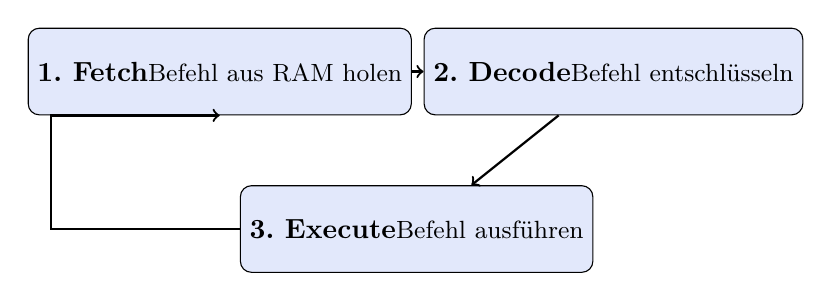
\begin{tikzpicture}[
        block/.style={draw, rounded corners, minimum width=3.5cm, minimum height=1.1cm, text centered, fill=RoyalBlue!15},
        arrow/.style={->, thick}
    ]
        \node[block] (fetch)   at (0, 0)    {\textbf{1.\ Fetch} \\ \small Befehl aus RAM holen};
        \node[block] (decode)  at (5, 0)    {\textbf{2.\ Decode} \\ \small Befehl entschlüsseln};
        \node[block] (execute) at (2.5,-2)  {\textbf{3.\ Execute} \\ \small Befehl ausführen};

        \draw[arrow] (fetch)   -- (decode);
        \draw[arrow] (decode)  -- (execute);
        \draw[arrow] (execute.west) -- ++(-2.4,0) |- (fetch.south);
    \end{tikzpicture}
    \caption{Der Fetch-Decode-Execute-Zyklus: die CPU wiederholt diesen Ablauf Milliarden Mal pro Sekunde.}
    \label{fig:fde}
\end{figure}

\begin{enumerate}
    \item \textbf{Fetch:} Das Steuerwerk liest den nächsten Befehl aus dem RAM an der Adresse, auf die der \emph{Programmzähler} (engl.\ \emph{program counter}) zeigt.
    \item \textbf{Decode:} Der Befehl wird in seine Bestandteile zerlegt: \emph{Was ist zu tun?} (z.\,B. Addieren) und \emph{Mit welchen Operanden?} (z.\,B. Register A und B).
    \item \textbf{Execute:} Die ALU oder eine andere Komponente führt die Anweisung aus (z.\,B. $A + B$), das Ergebnis wird in ein Register oder zurück in den Speicher geschrieben, und der Programmzähler rückt weiter.
\end{enumerate}

\begin{myexercise}
    Ein Prozessor hat eine Taktfrequenz von $3{,}6\,\mathrm{GHz}$ und führt im Durchschnitt 2 Befehle pro Taktzyklus aus.
    \begin{enumerate}
        \item Wie viele Befehle führt der Prozessor pro Sekunde aus?
        \item Ein Programm besteht aus $7{,}2 \times 10^9$ Befehlen. Wie lange dauert die Ausführung?
    \end{enumerate}
    \begin{myanswer}
        \begin{enumerate}
            \item $3{,}6 \times 10^9 \,\mathrm{Hz} \times 2 = 7{,}2 \times 10^9$ Befehle pro Sekunde.
            \item $\dfrac{7{,}2 \times 10^9}{7{,}2 \times 10^9\,\mathrm{s}^{-1}} = 1\,\mathrm{s}$.
        \end{enumerate}
    \end{myanswer}
\end{myexercise}
